%%% 
%% Project Management :: Planning 
%%% 
\section{Planning}
\label{sec:planning}

This section contains the project plans which have been developed in Microsoft
Project 2010. There are three sub sections which define the initial, interim and
final progress of the project. \citet{planning05} refers to software engineering
as two domains:

\begin{enumerate}
  \item Student Systems - Programs that people build to illustrate something or 
        for hobby.
  \item Industrial Strength Software - Software that can lead to significant 
        direct or indirect loss.
\end{enumerate}

A software project that is planned thoroughly is a more successful project than
a project that is developed through extreme programming. The Cryptic Crossword
project initially started through the Waterfall life cycle model and gradually
grew to become an Iterative model. Therefore the project plans had to be updated
constantly to reflect the change in which the project was being undertaken.

Although the overall project is developed in the Waterfall model due to the time
constraints applied by University deadlines the project consists of an iterative
development outside of the deliverables which are to be produced for academic
purposes.


\begin{landscape}

\subsection{Timeline}

\begin{figure}[H]
  \centering
  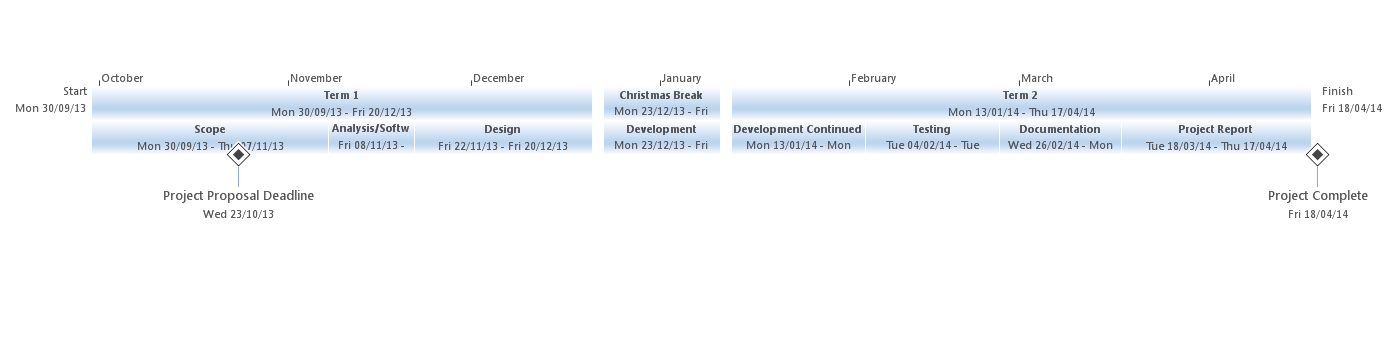
\includegraphics[width=\linewidth]{images/timeline1.png}
  \caption{Project Timeline (21$^s$$^t$ October 2013)}
  \label{fig:timeline1}
\end{figure}

Figure ~\ref{fig:timeline1} shows the initial time scale that was drawn up while
planning the project. This was produced to show the major deliverables and their
dates. In the next section the gantt Chart that was produced with all the
initial tasks to be completed are shown.

\newpage 
\subsection{Initial Gantt Chart}

\begin{figure}[H]
  \centering
  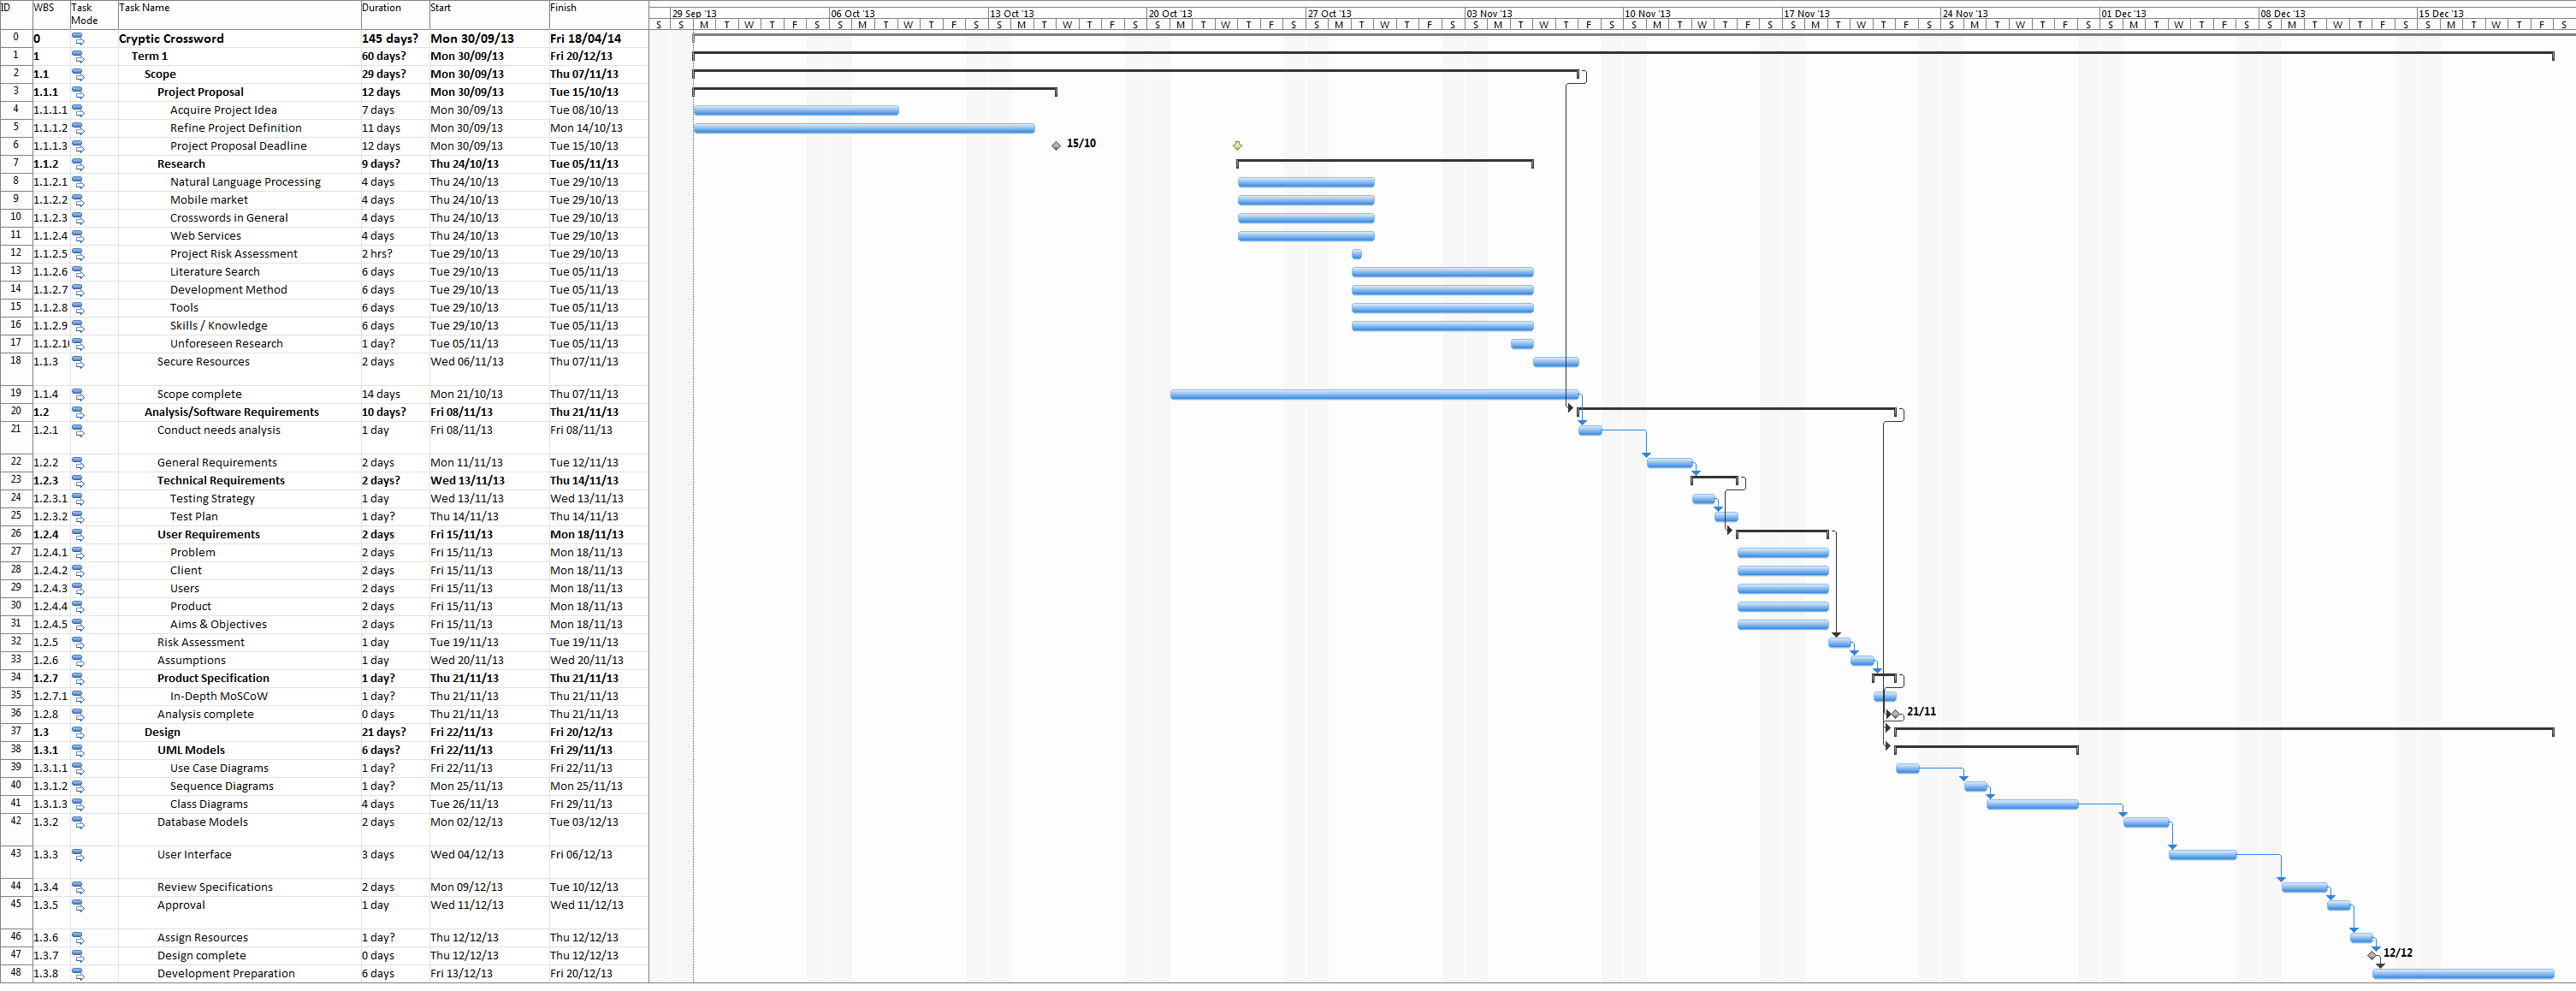
\includegraphics[width=\linewidth]{images/gant_chart1_term1.png}
  \caption{Gantt Chart for Term one (21$^s$$^t$ October 2013)}
  \label{fig:ganttinitialterm1}
\end{figure}

\begin{figure}[H]
  \centering
  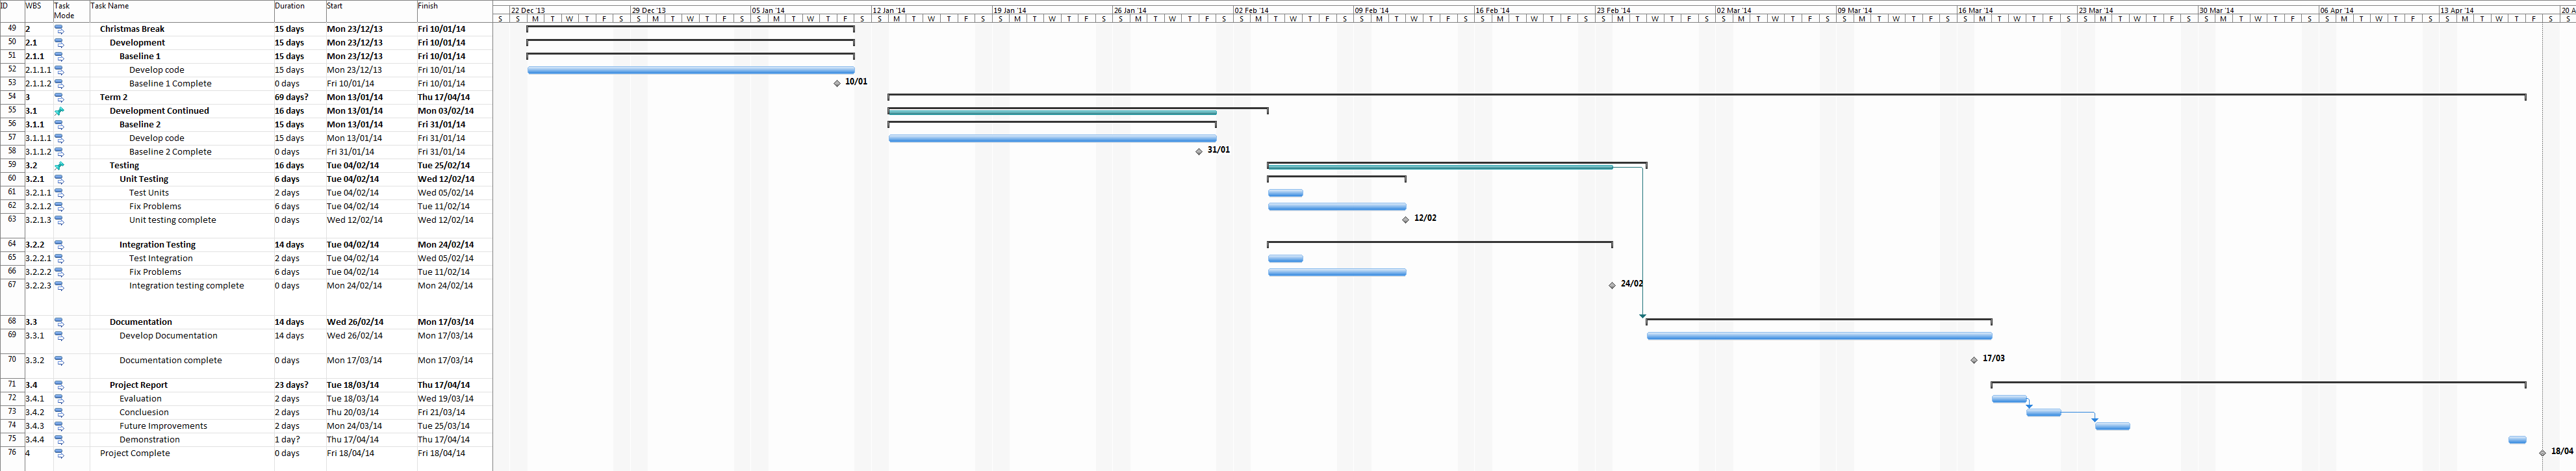
\includegraphics[width=\linewidth]{images/gant_chart1_term2.png}
  \caption{Gantt Chart for Term two (21$^s$$^t$ October 2013)}
  \label{fig:ganttinitialterm2}
\end{figure}

Figure ~\ref{fig:ganttinitialterm1} and ~\ref{fig:ganttinitialterm2} represent the initial lifecylce of the project. The gantt charts have been developed using the Waterfall model to allow the team members to work in flowing rhythm to ensure that all deliverables for the academic report are met. This includes the research and design for the project and at which point the team had a clearer understanding of the lifecycle the project is to incorporate.

\subsection{Timeline Re-Visited}

\begin{figure}[H]
  \centering
  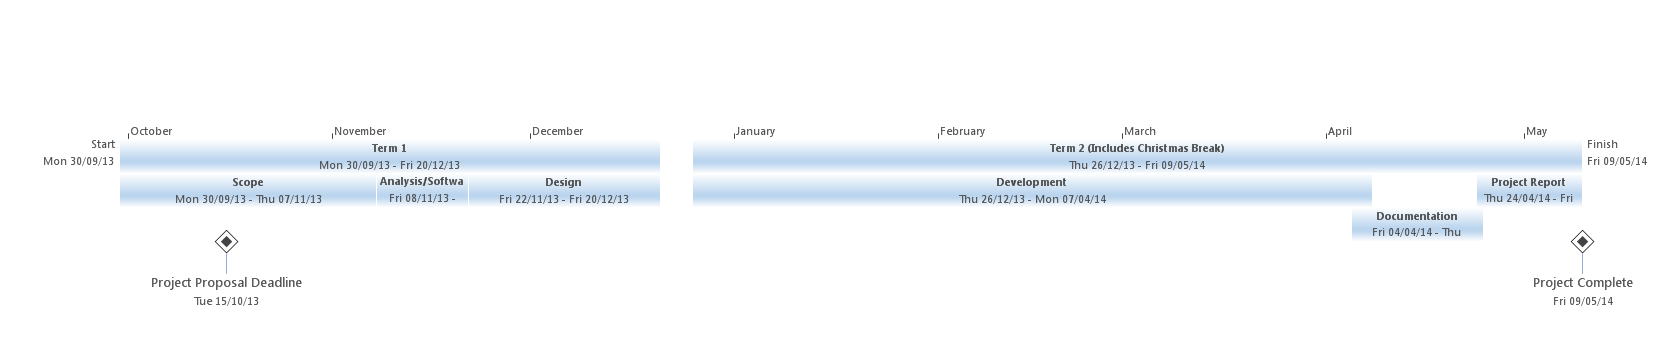
\includegraphics[width=\linewidth]{images/timeline2.png}
  \caption{Project Timeline (30$^t$$^h$ January 2014)}
  \label{fig:timeline2}
\end{figure}

By the end of term 1 the members of the group had accomplished all the back end research and acquired all the materials to start development of the project. At this point of the project new specifications were created and the research had implied that to develop such a system the best approach would be to take an iterative approach where some code can be developed and fully tested and deployed and then revisited to improve an another iteration. To ensure that a working system was developed and comprehensively tested it was decided that there was only sufficient time for three iterations. Although there would be three iterations it would allow a product to be submitted by the end of the second term and in the case the project ended early further iterations could be added in. Figure ~\ref{fig:timeline2} represents the new timeline which only focuses a change in the second term of the academic year and future tasks. 

\newpage 
\subsection{Interim Gantt Chart}

\begin{figure}[H]
  \centering
  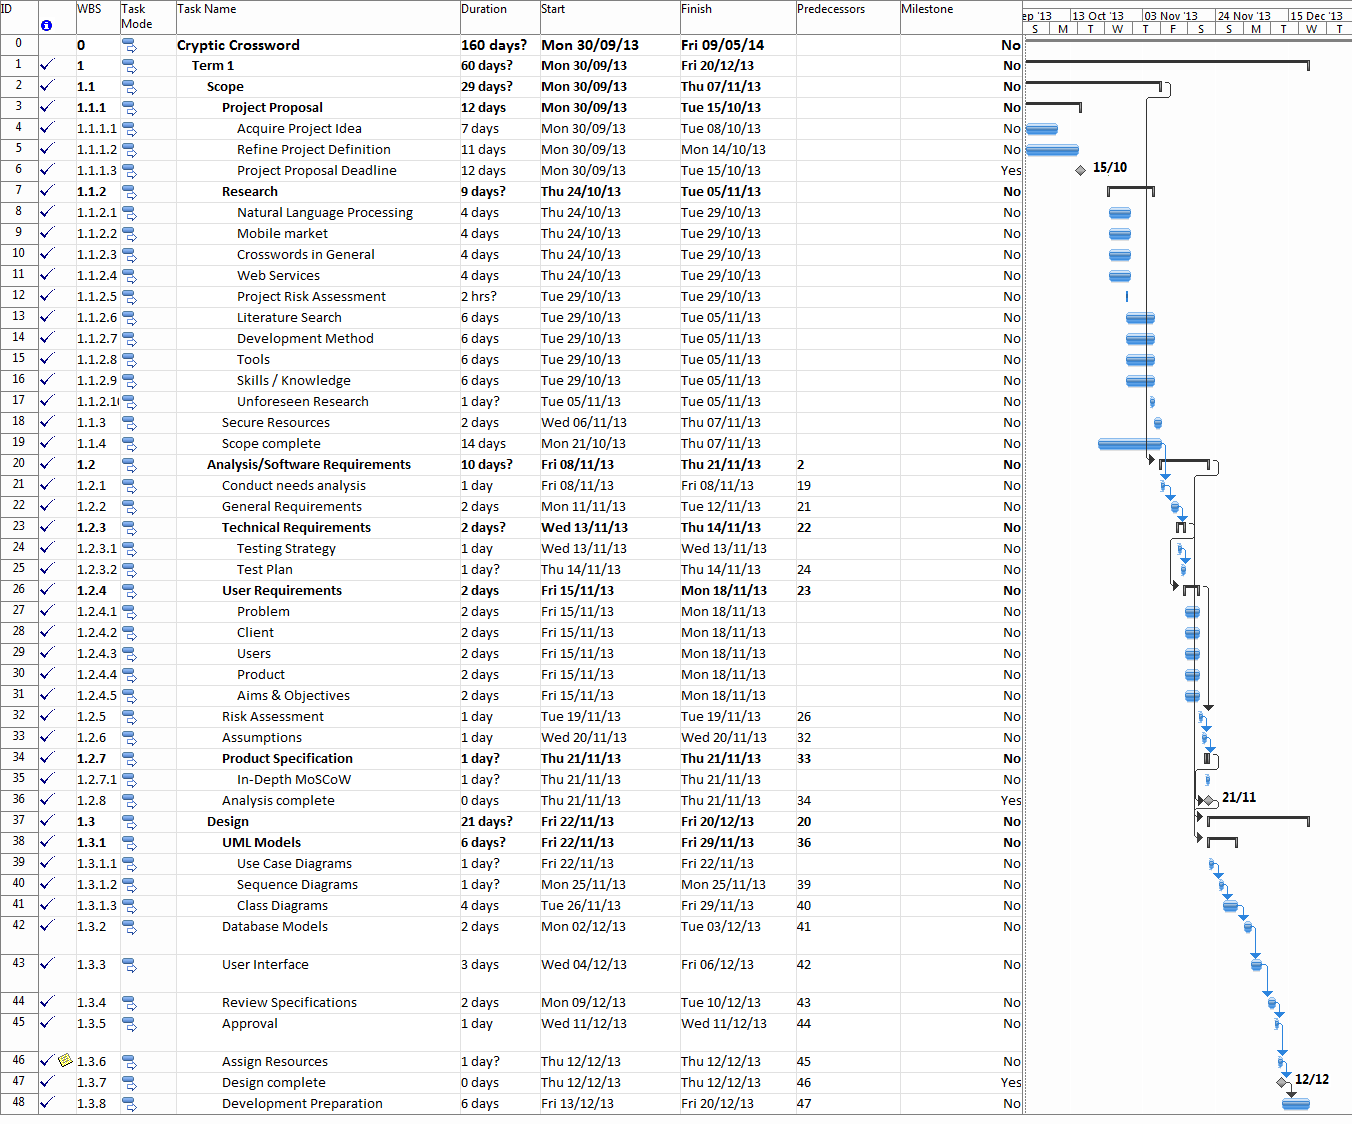
\includegraphics[scale=0.35]{images/gant_chart_interim_term1.png}
  \caption{Gantt Chart for Term one (30$^t$$^h$ January 2014)}
  \label{fig:ganttinterimterm1}
\end{figure}

\begin{figure}[H]
  \centering
  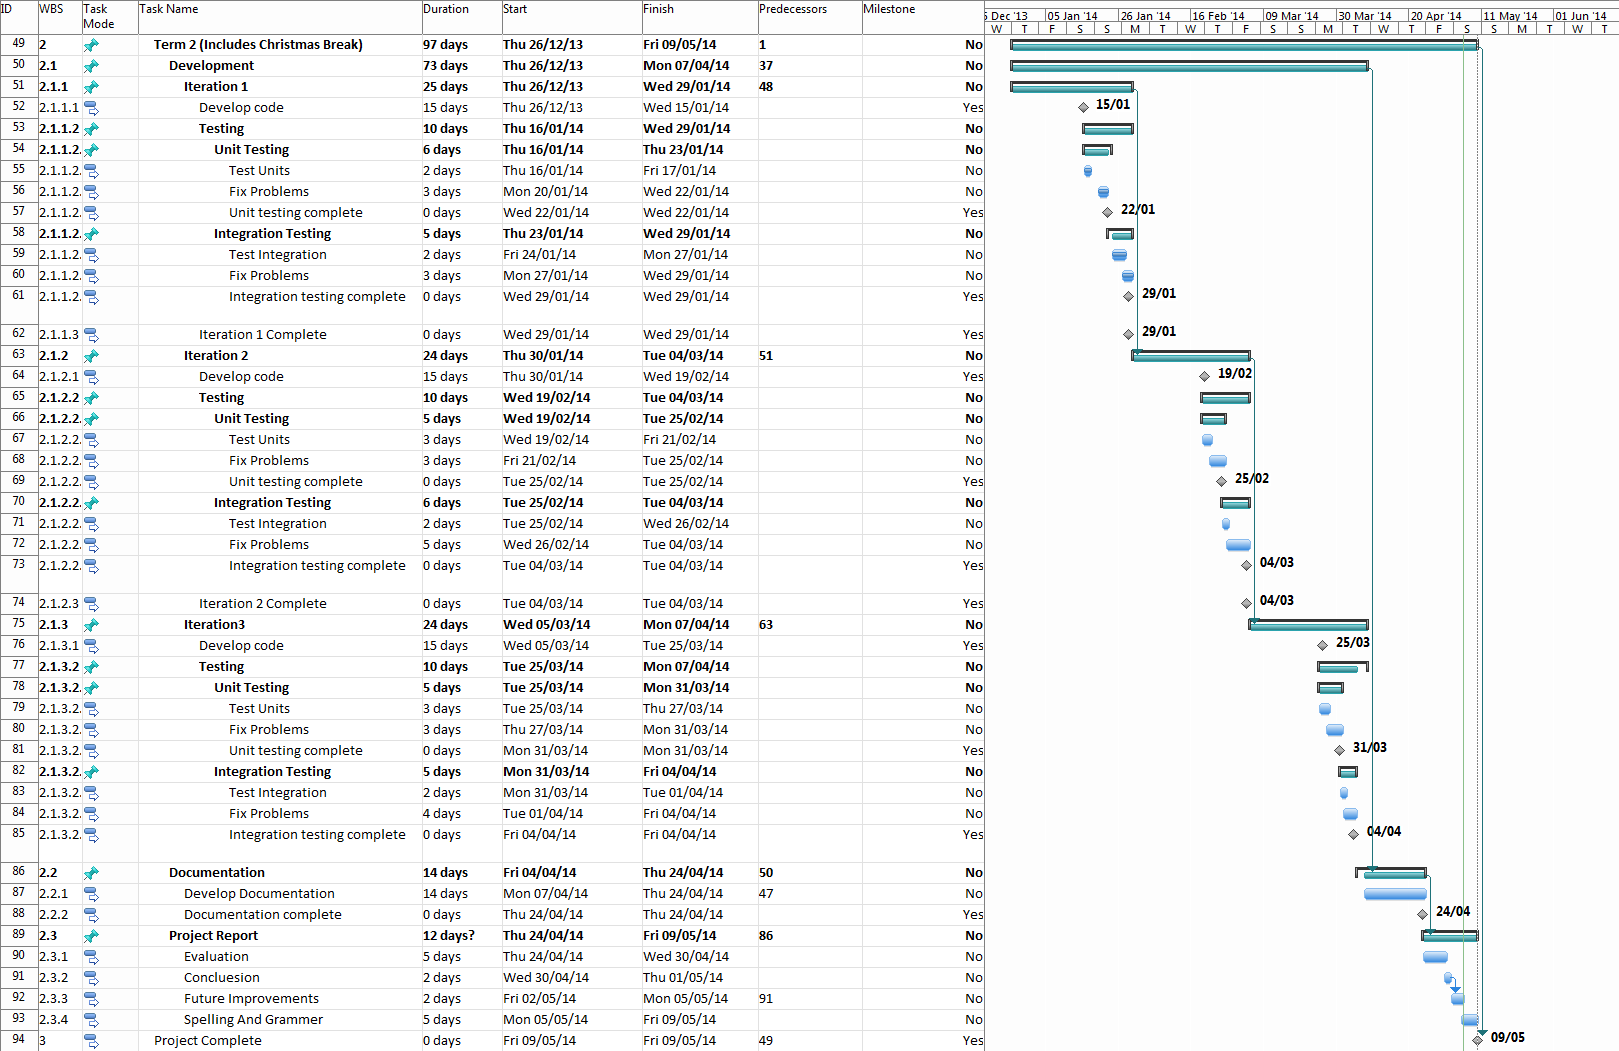
\includegraphics[width=\linewidth]{images/gant_chart_interim_term2.png}
  \caption{Gantt Chart for Term two (30$^t$$^h$ January 2014)}
  \label{fig:ganttinterimterm2}
\end{figure}

Figure ~\ref{fig:ganttinterimterm2} shows the flow of the new tasks that incorporate the Iterative development model and the remaining tasks of the second term. The Work Breakdown Structure(WBS) ensures that tasks are started only when tasks are completed and have a must finish on constraint to ensure that work is completed on time. Weekends have been excluded from the work hours to allow team members to work on other modules from their university studies as well as time off for social activities.


\subsection{Final Gantt Chart}

\begin{figure}[H]
  \centering
  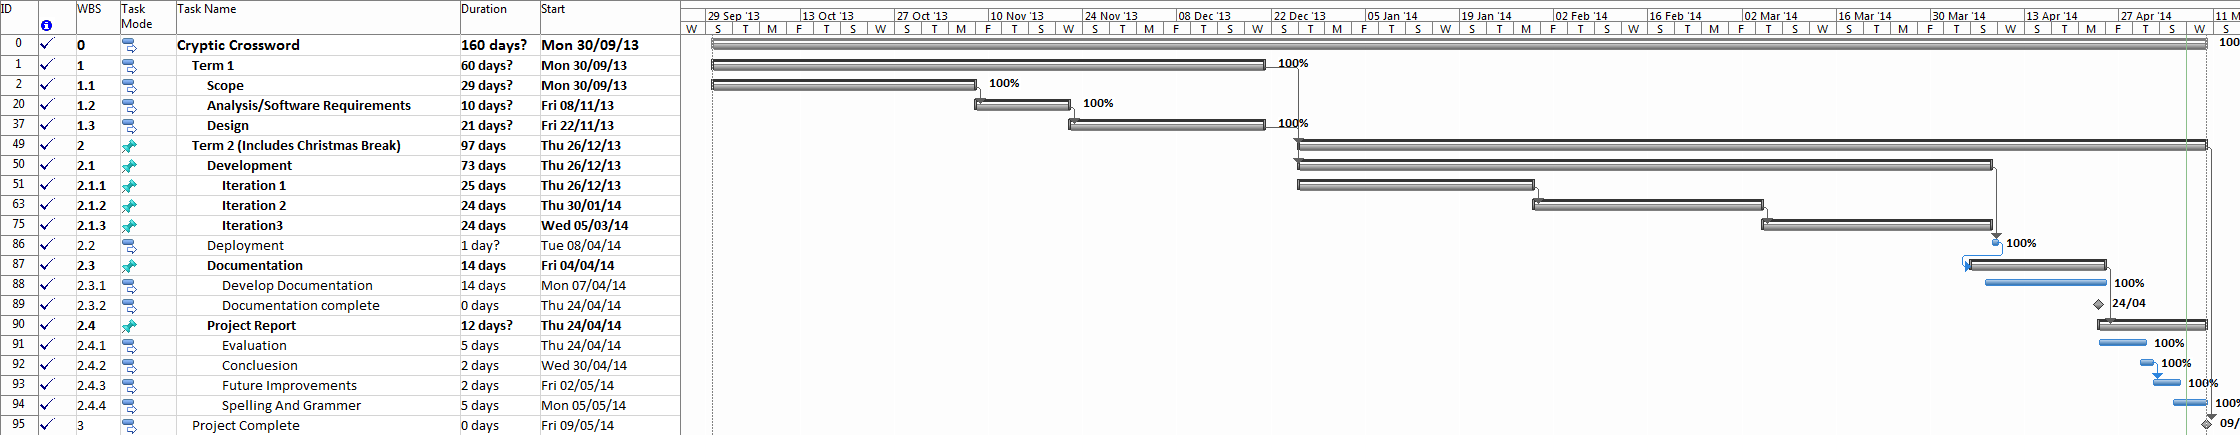
\includegraphics[width=\linewidth]{images/gant_chart_final_overview.png}
  \caption{Final Gantt Chart of Project Summary (7$^t$$^h$ May 2014)}
  \label{fig:ganttfinaloverview}
\end{figure}

\begin{figure}[H]
  \centering
  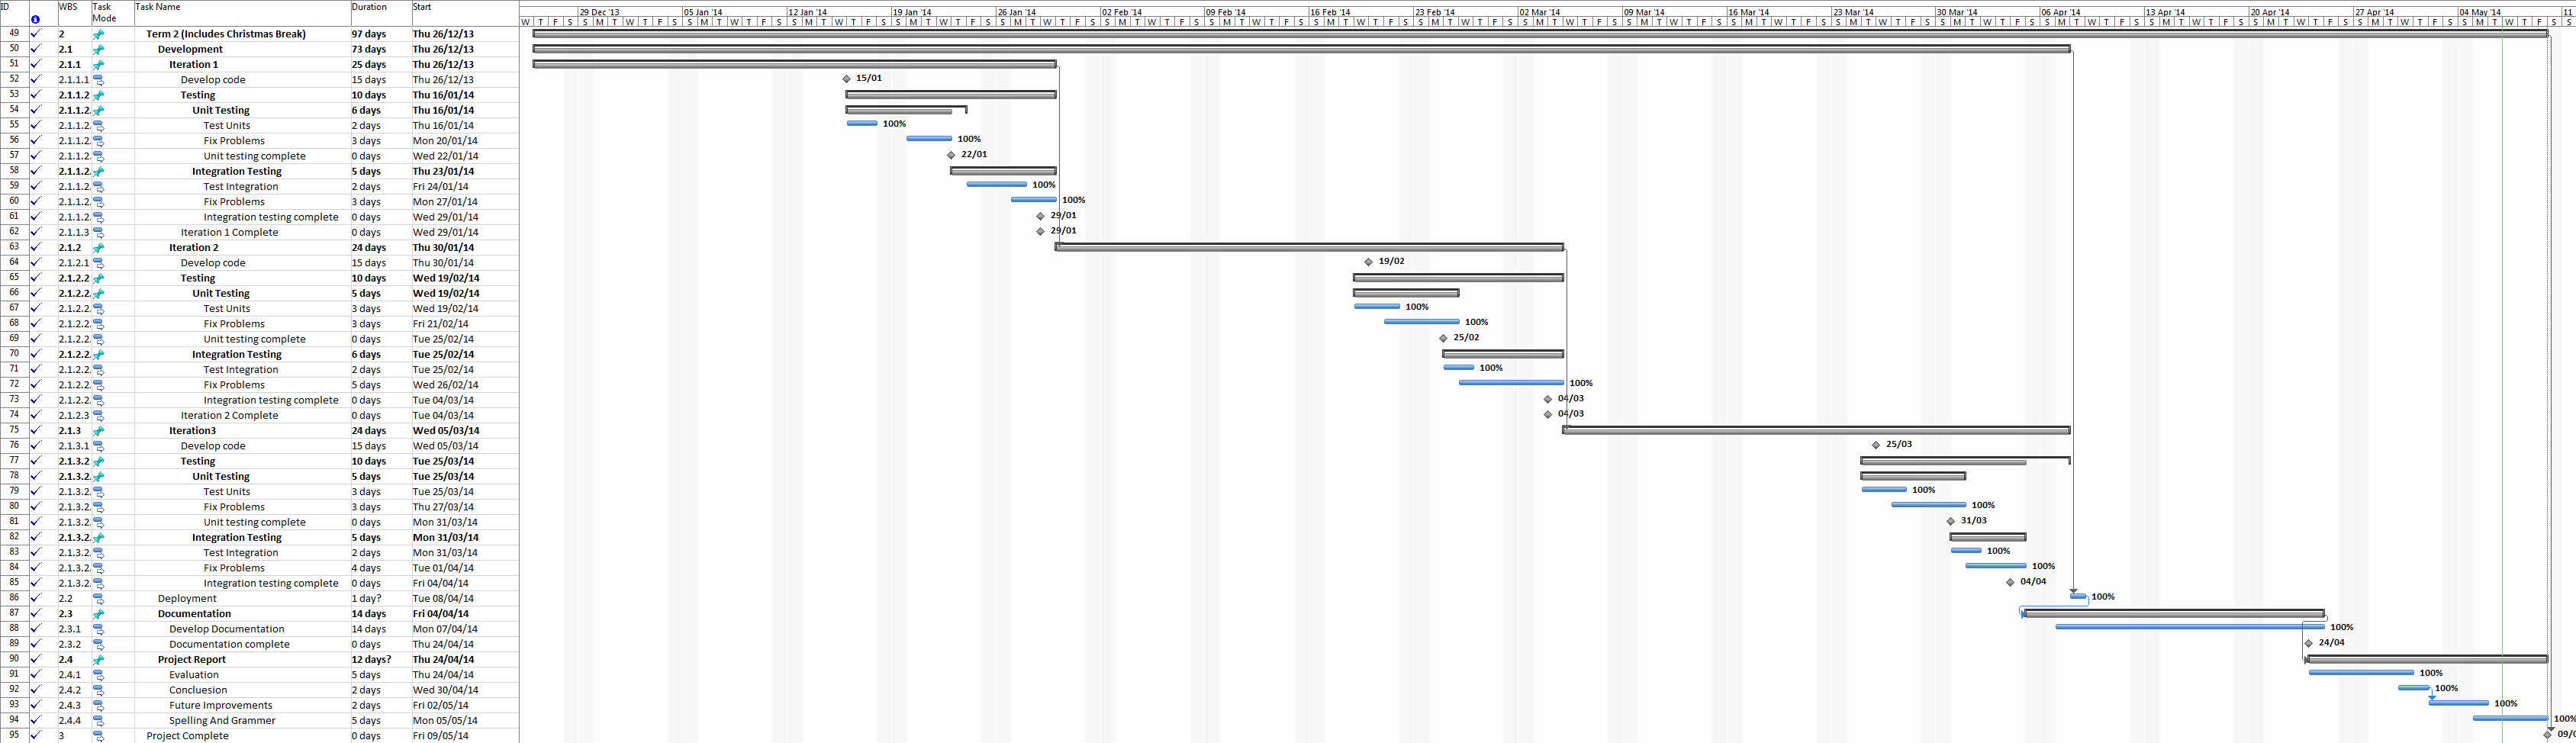
\includegraphics[width=\linewidth]{images/gant_chart_final_term2.png}
  \caption{Final Gantt Chart for Term two (7$^t$$^h$ May 2014)}
  \label{fig:ganttfinalterm2}
\end{figure}

Figure ~\ref{fig:ganttfinalterm2} is the final gantt chart for the second term. Al tasks have been completed on time and a product has been deployed on the web server. Improvements have been identified but there is not enough time for a fourth iteration. Figure ~\ref{fig:ganttfinaloverview} represents an overview of the two terms and the milestones completed.

\end{landscape}
